\documentclass[10pt]{article}
\usepackage[letterpaper,margin=0.75in]{geometry}
\usepackage[T1]{fontenc}
\usepackage{lmodern,microtype,graphicx,booktabs,amsmath,enumitem,needspace}
\usepackage[hidelinks]{hyperref}
\makeatletter\long\def\@makecaption#1#2{\vskip3pt{\small\textbf{#1.} #2\par}}\makeatother
\setlength{\parindent}{0pt}\setlength{\parskip}{4pt}
\setlist{nosep,leftmargin=*}
\renewcommand{\section}[1]{\needspace{5\baselineskip}\vspace{5pt}{\large\bfseries #1\par}\vspace{1pt}}
\pagestyle{plain}

\begin{document}
{\Large\bfseries Forecasting small-business AI use six weeks ahead}\\[2pt]
ISYE 4031 Milestone 2 \textbullet{} Group 1 \textbullet{} October 2026\\
Rahul Mehta, Ishaan Mohan, Zhengyu Chris Liu, Timothy Kim, Chau M Duong

\section{1. Question and response to feedback}
\textbf{Question.} Can a regression forecast an industry-by-size group's AI-use rate three Census releases (about six weeks) ahead more accurately than simple historical forecasts, and is it reliable enough to guide outreach planning?
\textbf{Target:} the published percentage of employer businesses in a group that used AI in the last two weeks (Census BTOS). Small business means 1--99 employees.
\textbf{Use:} deciding which industries and firm sizes to prioritize for AI outreach. The forecast describes groups, not firms, and says nothing about the effect of outreach.

\textbf{Feedback and response.}
\begin{itemize}
\item \emph{TA, Milestone 1:} define the target and model, use several predictors, fit a baseline, and respect the short history. We state the model (Section 4), use current rate, industry, size, and trend, compare two naive forecasts, and evaluate only in time order.
\item \emph{October 20 meeting (relayed by Chris):} compare industries and show uncertainty. We added industry growth estimates with intervals (Figure 1) and separate regressions per industry.
\item \emph{October 27--28 (professor, relayed by Chris):} consider AI model-release timing, benchmark scores, and a nonstationary Poisson process. We ran exploratory versions (Section 5). The exact scope of this request is not yet confirmed.
\end{itemize}

\section{2. Data and preparation}
\textbf{Source.} Census Business Trends and Outlook Survey, sector-by-employment-size workbook, downloaded October 20, 2026 and hashed. One observation is a NAICS sector $\times$ size band in one biweekly release. Variables: AI-use rate and expected-use rate (\%), the rate's standard error (SE, percentage points), sector, size band, release, and publication date. We use the 23 releases from the November 2025 question revision (202524) through release 202620, published October 8, 2026; earlier releases asked a narrower question.

\begin{tabular}{@{}lr@{}}
\toprule
Pipeline step & Count\\\midrule
Published cells: 20 sectors $\times$ 5 size bands $\times$ 23 releases & 2{,}300\\
Suppressed by Census, kept as missing (not imputed) & 519 (22.6\%)\\
Groups kept: rate and expected use in $\ge$7 of the first 8 releases & 71 groups, 15 industries\\
Issue--target pairs ($t \to t{+}3$), complete cases & 1{,}406\\
Scored forecasts: 10 issue dates, April 23 -- August 27, 2026 & 706\\\bottomrule
\end{tabular}

\textbf{Quality.} No duplicate group-release keys; all rates lie in 0--100. Suppression is 20--25\% in every size band. Survey noise rises with firm size: the median SE of a forecast target is 1.7 pp for 1--4 employees and 5.2 pp for 50--99. The 50--99 band keeps only 11 of 15 industries. An earlier third-party extract of the same data matches this workbook exactly on all 1{,}781 rates, 1{,}825 expected-use rates, 1{,}781 SEs, and missingness; one publication date differs by a day (release 202526) and does not affect any forecast.

\textbf{Dependence and leakage.} The same 71 groups recur every release, and a new BTOS sample year began with release 202616 (collected from July 27, 2026), so the 706 forecasts share 10 dates and common shocks; they are not independent. A forecast is issued on release $t$'s publication date. Training uses only pairs whose target was already published; screening uses only the first 8 releases; preprocessing is fit on training rows. The code asserts these rules, and we confirmed them with an independent refit.

\section{3. Exploratory findings}
\begin{figure}[h]\centering
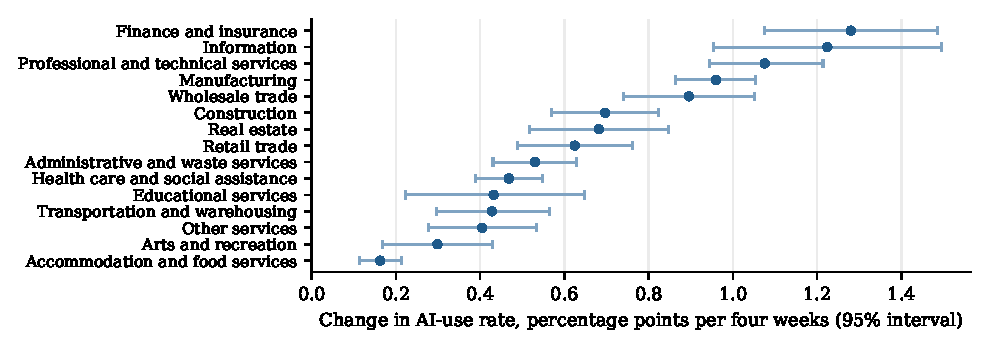
\includegraphics[width=\linewidth]{figures/fig1_industry_growth.pdf}
\caption{Estimated growth in AI use by industry, 71 groups, releases 202524--202620. Intervals: 95\% moving-block bootstrap (2{,}000 draws). They describe this period and are conditional on the model; they are not forecasts.}
\end{figure}
\vspace{-6pt}
Adoption rose in every industry, but at very different speeds. Finance, Information, and Professional services grew about 1.1--1.3 pp per four weeks; Accommodation and food grew 0.16. The top three are clearly separated from the rest (each is in the bootstrap top three in $\ge$97\% of draws), but their order is not. This motivated separate industry models: one pooled trend under-forecasts the fast industries and over-forecasts the slow ones.

The second pattern is noise. A 50--99 estimate can move about 10 pp (two SEs) with no real change. No model can forecast below this floor, so we judge errors against the target's SE (Figure 2).

\section{4. Baseline and results}
\textbf{Baseline.} Pooled ordinary least squares for group $g$ at issue release $t$:
\[ y_{g,t+3} = \beta_0 + \beta_1 y_{g,t} + \alpha_{\text{industry}} + \gamma_{\text{size}} + \beta_2 t + \varepsilon_{g,t+3}. \]
Every term is known at issue. \textbf{References:} carry the latest rate forward; mean of the group's latest six releases. \textbf{Extension:} the same equation fit separately within each industry. \textbf{Validation:} expanding window, refit at each of 10 issue dates, horizon three releases. \textbf{Metric:} mean absolute error (MAE) in pp; RMSE penalizes large misses. Differences are averaged over dates, with 95\% moving-block bootstrap intervals over dates.

\begin{table}[h]\centering\small
\begin{tabular}{@{}lccccc@{}}
\toprule
Forecast & MAE & RMSE & Bias & Change vs.\ six-release mean [95\% CI] & Better at \\\midrule
Carry latest rate forward & 4.15 & 5.75 & $-1.05$ & --- & --- \\
Six-release mean & 3.39 & 4.64 & $-2.07$ & reference & --- \\
\textbf{Pooled regression (baseline)} & \textbf{3.30} & \textbf{4.55} & $+0.07$ & $-0.09$ [$-0.22$, $+0.04$] & 7 of 10 dates \\
Separate industry regressions$^\dagger$ & 3.04 & 4.29 & $-0.21$ & $-0.35$ [$-0.46$, $-0.24$] & 9 of 10 \\
Gradient boosting$^\dagger$ & 3.08 & 4.33 & $-0.45$ & $-0.31$ [$-0.42$, $-0.22$] & 10 of 10 \\
Unregularized regression, all predictors$^\dagger$ & 6.01 & 8.15 & $+3.44$ & $+2.61$ [$+0.30$, $+5.86$] & 1 of 10 \\\bottomrule
\end{tabular}
\caption{Out-of-sample error (pp), 706 forecasts at 10 issue dates. $^\dagger$Designed after these outcomes were published; a retrospective result, not a test.}
\end{table}
\vspace{-4pt}
\begin{figure}[h]\centering
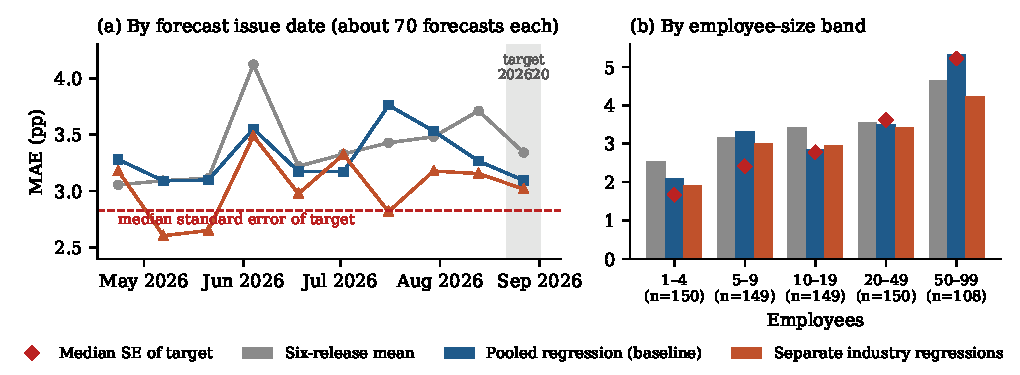
\includegraphics[width=\linewidth]{figures/fig2_errors.pdf}
\caption{Forecast MAE (a) at each issue date and (b) by size band. Red: median SE of the published target, a floor set by survey noise. Shaded: forecasts of release 202620, issued August 27.}
\end{figure}
\vspace{-6pt}
\textbf{Results.} The baseline beats carrying the rate forward by 0.85 pp but beats the six-release mean by only 0.09 pp, and the interval includes zero. Its main gain is removing bias: the six-release mean lags a rising trend by 2.1 pp. In the original 9-date evaluation, the last fit's coefficient on the current rate is 0.21, so the model behaves like a smoothed group average plus a trend. Expected use added nothing (MAE 3.33 vs.\ 3.33 in the 9-date original evaluation).
Separate industry models cut MAE by 0.35 pp (10\%) against the six-release mean and 0.26 pp against the baseline, and win at 9 of 10 dates. That is the only gain whose interval excludes zero, but we chose that design after seeing these outcomes and tried several alternatives, so the gain is likely overstated.

\textbf{Diagnostics} (original 9-date evaluation). Residuals fan out as fitted rates rise. The four largest Cook's distances all belong to Information firms with 50--99 employees (residuals up to 27 pp), but none is highly influential (maximum 0.08); dropping the five most influential rows made last-date MAE worse (3.27 to 3.37), so we kept them. Errors track survey noise: 84\% of baseline errors are within two SEs of the target, and absolute error correlates with target SE ($r = 0.44$). In the 50--99 band, the three methods in Figure 2 miss by 4.2--5.3 pp on average.

\textbf{One forward check.} The baseline was fixed before release 202620 was published (October 8). On those 71 forecasts its MAE is 3.09, against 3.34 for the six-release mean and 3.90 for carry-forward. One date is not enough to confirm the ranking.

\section{5. Preliminary answer, limitations, next steps}
\textbf{Answer.} Partly. Six weeks ahead, simple models forecast group AI use to within about 3 pp, close to the survey's own noise (2.8 pp). The pooled baseline is not reliably better than a six-release average. Separate industry models look better, but that result is retrospective. Forecasts are usable to rank industries for outreach, where Figure 1's separation is clear; they are not reliable enough to target individual size bands, especially 50--99 employees.

\textbf{Limitations.} (1) Short history: 10 forecast dates with shared shocks, so intervals are wide and fragile. (2) Model selection after outcomes were known. (3) Survey noise, suppression, and screening: results cover 71 well-measured groups, not all small businesses or nonemployers. (4) One downloaded vintage; we cannot prove earlier values were unrevised at each forecast date. (5) Association only: industry differences and adoption trends are not causal.

\textbf{Exploratory work on AI releases (not used in forecasts).} With Epoch AI's model catalogue (1{,}045 language models, January 2024--September 2026), a log-linear (nonstationary) Poisson rate forecast monthly counts with MAE 8.6 models vs.\ 12.6 for a constant rate over 21 months. For GPQA Diamond best scores, carrying the last value forward beat a six-month trend (MAE 0.55 vs.\ 2.10 points, 7 comparisons). Catalogue dates are recorded after the fact and need not match public release, and we have not linked either series to adoption. Neither shows that model releases drive adoption.

\textbf{Most important for Milestone 3.} Freeze the industry model now and score it on releases published after this report, before looking at those outcomes.

\section{6. Team contributions and reflection}
\textbf{Contributions.} All five members contributed equally. Chris built the industry and nonlinear forecasting extension; Rahul audited the official workbook, ran the release and benchmark explorations, and assembled the report. \textbf{[Team to confirm before submission: Ishaan's, Timothy's, and Chau's specific work.]}

\textbf{What we learned.} Aggregate accuracy hid failures: the baseline wins overall but loses in two size bands. Survey noise sets a floor no model can beat. Testing in time order, and only on outcomes published after the model was fixed, is what separates a forecast from a fit.

\textbf{What failed or changed.} Our Milestone 1 hypothesis, that regression beats the six-release mean at most dates and in every size band, was not supported for the pooled baseline. Expected use and business-performance predictors did not help. A regression with every predictor overfit (MAE 6.01). Nonlinear terms gave no gain.

\begin{tabular}{@{}ll@{}}
\toprule
Next-stage task & Owner\\\midrule
Freeze industry model; prospective test on new releases & \textbf{[to confirm]}\\
Confirm professor's scope for release, benchmark, and Poisson work & \textbf{[to confirm]}\\
Define the outreach decision and the cost of a forecast miss & \textbf{[to confirm]}\\
Calibrate forecast intervals by size band & \textbf{[to confirm]}\\\bottomrule
\end{tabular}

\textbf{AI use.} AI tools, including Anthropic's Claude, helped write and debug analysis code, check results against the data, and draft and edit this report. All numbers come from the submitted code. The team is responsible for every claim.

{\footnotesize\textbf{Sources.} U.S. Census Bureau, Business Trends and Outlook Survey, Sector by Employment Size Class workbook and methodology, census.gov/hfp/btos. Epoch AI, Data on AI Models and Benchmarking data, epoch.ai/data. Code: github.com/chris-zy-liu/regression-project.\par}
\end{document}
